\documentclass[11pt]{article}

\usepackage[utf8]{inputenc}
\usepackage[portuges]{babel}
\usepackage{indentfirst}
\usepackage{natbib}
\usepackage{graphicx}
\usepackage{geometry}
 \geometry{
    a4paper,
    total={130mm,227mm},
    left=40mm,
    top=40mm,
}
 
\renewcommand{\contentsname}{Índice}

\begin{document}

\begin{titlepage}
    \begin{center}
        
\includegraphics[width=0.3\textwidth]{images/capa/EscolaEngenhariaUM.jpeg}
    
        \vspace{1cm}
        
        \textbf{\LARGE Redes de Computadores}
    
        \vspace{0.5cm}
        \textbf{\Large Trabalho Prático 4}

        \vspace{1.3cm}
        
        \textbf{\large Francisco Correia Franco A89458 \\
        António Jorge Nande Rodrigues A89585 \\
        Luís Enes Sousa A89597}

        \vspace{1.5cm}
    
        \begin{figure}[hbt!]
        \minipage{0.32\textwidth}
            
\includegraphics[width=\linewidth]{images/capa/152.png}
            \centering
            \captionsetup{A89458}
        \endminipage\hfill
        \minipage{0.32\textwidth}
            
\includegraphics[width=\linewidth]{images/capa/133.jpeg}
            \centering
            \captionsetup{A89585}
        \endminipage\hfill
        \minipage{0.32\textwidth}
            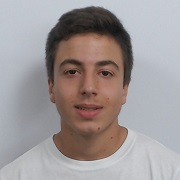
\includegraphics[width=\linewidth]{images/capa/80.jpeg}
            \centering
            \captionsetup{A89597}
        \endminipage
        \end{figure}
    \end{center}
\end{titlepage}

\tableofcontents
\thispagestyle{empty}
\cleardoublepage

\setcounter{page}{1}


%-----------------------------------------------------------------%
\section{Acesso Rádio}

Como pode ser observado, a sequência de bytes capturada inclui informação do nível físico (radio information), para além dos bytes correspondentes a tramas 802.11.

Para a trama correspondente 352:

\begin{figure}[hbt!]
    \centering
    \frame{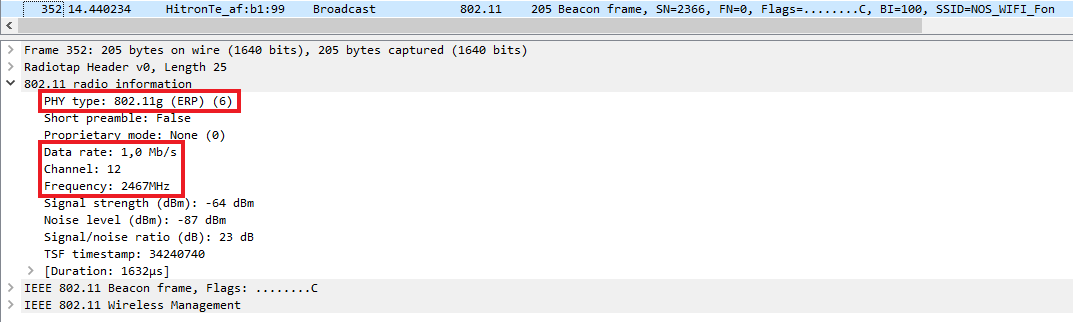
\includegraphics[width=1\textwidth]{images/cap4/trama_352.png}}
    \caption{Trama 352}
\end{figure}

\subsection{Pergunta 1}

\textbf{Identifique em que frequência do espectro está a operar a rede sem fios, e o canal que corresponde essa frequência.}

A rede sem fios está a operar na frequência 2467 MHz, correspondente ao canal 12.

\subsection{Pergunta 2}

\textbf{Identifique a versão da norma IEEE 802.11 que está a ser usada.}

A versão que está a ser usada é a 802.11g.

\subsection{Pergunta 3}

\textbf{Qual o débito a que foi enviada a trama escolhida? Será que esse débito corresponde ao débito máximo a que a interface WiFi pode operar? Justifique.}

A trama foi enviada a um débito de 1 Mb/s.

Ese débito não corresponde ao débito máximo a que a interface WiFi pode operar, pois esta suporta um débito de até 54 Mb/s.


%-----------------------------------------------------------------%
\clearpage
\section{Scanning Passivo e Scanning Ativo}

Como referido, as tramas beacon permitem efetuar scanning passivo em redes IEEE 802.11 (WiFi). Para a captura de tramas disponibilizada, responda às seguintes questões:

\vspace{0.5cm}

\subsection{Pergunta 4}

\textbf{Selecione uma trama beacon (e.g., trama 1052). Esta trama pertence a que tipo de tramas 802.11? Indique o valor dos seus identificadores de tipo e de subtipo. Em que parte concreta do cabeçalho da trama estão especificados (ver anexo)?}

As tramas Beacon pertencem ao tipo de tramas de Gestão (Management frames). Os valores dos seus identificadores de tipo e de subtipo são, respetivamente, 0 e 8.

Estes identificadores estão especificados no byte 0x19 do cabeçalho. Mais especificamente, o identificador de subtipo encontra-se nos 4 bits mais significativos e o de tipo nos 2 bits seguintes.

\begin{figure}[hbt!]
    \centering
    \frame{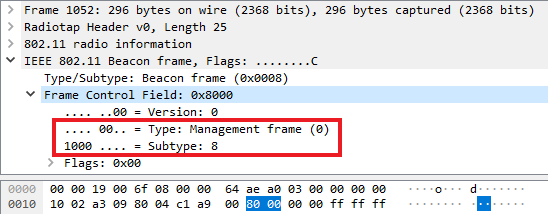
\includegraphics[width=.5\textwidth]{images/cap5/tipo_subtipo_1052.png}}
    \caption{Tipo e subtipo da trama 1052}
\end{figure}

\subsection{Pergunta 5}

\textbf{Para a trama acima, identifique todos os endereços MAC em uso. Que conclui quanto à sua origem e destino?}

Estão em uso 3 endereços MAC: recetor ou destino (ff:ff:ff:ff:ff:ff - Broadcast), transmissor ou origem (bc:14:01:af:b1:98 - HitronTe\_af:b1:98) e BSS Id (bc:14:01:af:b1:98 - HitronTe\_af:b1:98).

Concluímos que a trama teve origem no dispositivo bc:14:01:af:b1:98 (HitronTe\_af:b1:98) e destino nos vários dispositivos ligados à rede.

\begin{figure}[hbt!]
    \centering
    \frame{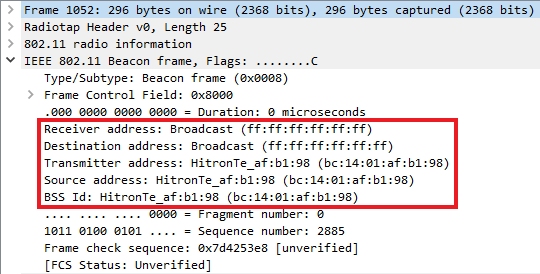
\includegraphics[width=.5\textwidth]{images/cap5/enderecosMAC_1052.png}}
    \caption{Endereços MAC na trama 1052}
\end{figure}

\subsection{Pergunta 6}

\textbf{Uma trama beacon anuncia que o AP pode suportar vários débitos de base, assim como vários débitos adicionais (extended supported rates). Indique quais são esses débitos?}

Os débitos de base suportados são 1, 2, 5.5, 11, 9, 18, 36 e 54 Mb/s.

Os débitos adicionais suportados são 6, 12, 24, 48 Mb/s.

\begin{figure}[hbt!]
    \centering
    \frame{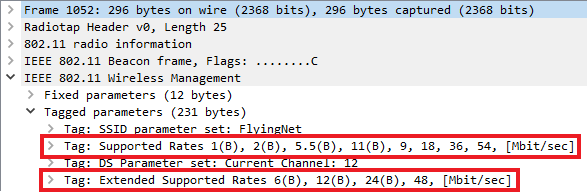
\includegraphics[width=.5\textwidth]{images/cap5/debitos_1052.png}}
    \caption{Débitos de base e adicionais da trama 1052}
\end{figure}

\subsection{Pergunta 7}

\textbf{Qual o intervalo de tempo previsto entre tramas beacon consecutivas? (nota: este valor é anunciado na própria trama beacon). Na prática, a periodicidade de tramas beacon provenientes do mesmo AP é verificada? Tente explicar porquê.}

O intervalo de tempo previsto entre tramas beacon consecutivas é 0.1024 segundos.

\begin{figure}[hbt!]
    \centering
    \frame{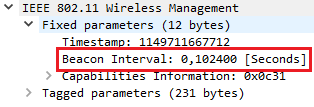
\includegraphics[width=0.4\textwidth]{images/cap5/beacon_interval_1052.png}}
    \caption{Intervalo de tempo previsto entre duas tramas Beacon}
\end{figure}

Na prática, a periodicidade não se verifica, embora seja por meras frações de segundo. Isto pode dever-se ao facto de existir tráfego associado ao Access Point. No exemplo da figura seguinte os intervalos observados são 0,102314 e 0,102538 segundos.

\begin{figure}[hbt!]
    \centering
    \frame{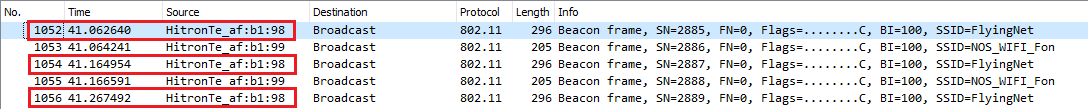
\includegraphics[width=1\textwidth]{images/cap5/beacon_interval_pratico.png}}
    \caption{Intervalo de tempo prático entre três tramas Beacon}
\end{figure}
\clearpage
\subsection{Pergunta 8}

\textbf{Identifique e liste os SSIDs dos APs que estão a operar na vizinhança da STA de captura? Explicite o modo como obteve essa informação (por exemplo, se usou algum filtro para o efeito).}

Pela observação de algumas tramas Beacon consecutivas, verficamos que existe um padrão de alternância entre dois APs. Isto significa que estão a operar dois APs na vizinhança da STA de captura, sendo os seus SSIDs 'FlyingNet' e 'NOS\_WIFI\_Fon'.

\begin{figure}[hbt!]
    \centering
    \frame{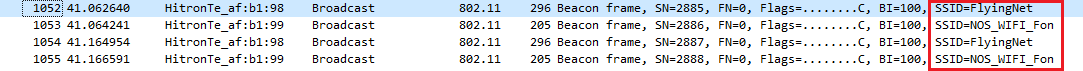
\includegraphics[width=1\textwidth]{images/cap5/SSIDs_dos_APs.png}}
    \caption{SSIDs dos APs na vizinhança da STA de captura}
\end{figure}

\subsection{Pergunta 9}

\textbf{Verifique se está a ser usado o método de deteção de erros (CRC). Justifique.}

Na figura seguinte verificamos que está presente um campo FCS na trama 1052. Isto significa que está a ser usado um método de deteção de erros.

\begin{figure}[hbt!]
    \centering
    \frame{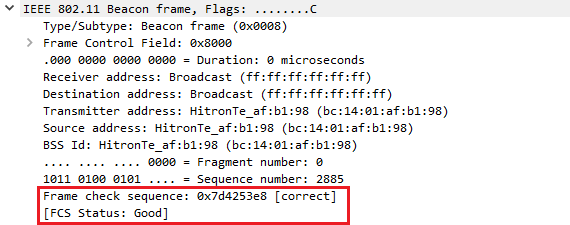
\includegraphics[width=0.6\textwidth]{images/cap5/fcs_1052.png}}
    \caption{Campo FCS (Frame Check Sequence) na trama 1052}
\end{figure}

Através do uso do filtro '(wlan.fc.type\_subtype == 0x08) && (wlan.fcs.status == bad)' conseguimos verificar que houve erros no envio de algumas tramas Beacon. Isto confirma a necessidade de usar deteção de erros em redes sem fios, pois estas são muito menos estáveis que, por exemplo, redes Ethernet.

\begin{figure}[hbt!]
    \centering
    \frame{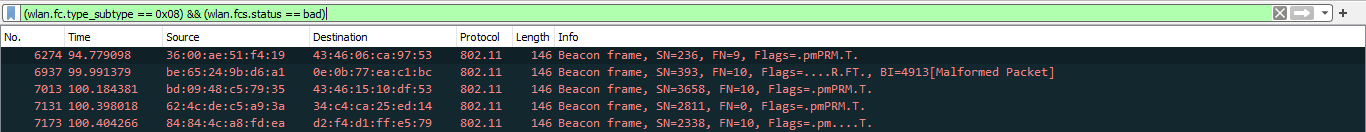
\includegraphics[width=1\textwidth]{images/cap5/filtro_fcs_status_bad.png}}
    \caption{Filtro para detetar tramas Beacon com erros}
\end{figure}


No trace disponibilizado foi também registado scanning ativo (envolvendo tramas probe request e probe response), comum nas redes Wi-Fi como alternativa ao scanning passivo. 

\subsection{Pergunta 10}

\textbf{Estabeleça um filtro Wireshark apropriado que lhe permita visualizar todas as tramas probing request ou probing response, simultaneamente.}

O filtro 'wlan.fc.type\_subtype == 4 or wlan.fc.type\_subtype == 5' limita as tramas apresentadas àquelas cujo subtipo é igual a 4 ou 5 (probing request ou probing response, respetivamente).

\begin{figure}[hbt!]
    \centering
    \frame{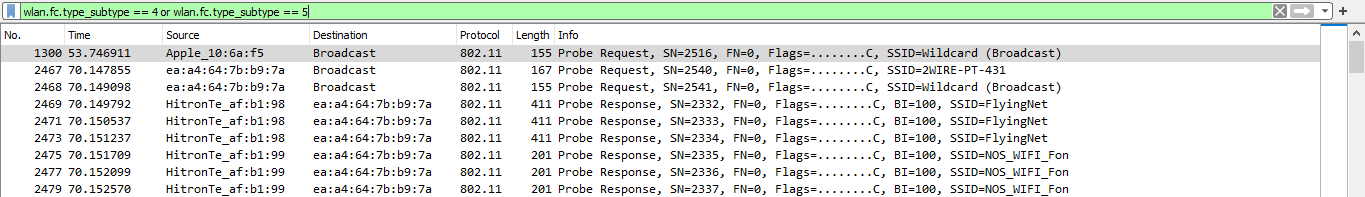
\includegraphics[width=1\textwidth]{images/cap5/filtro_estabelecido.png}}
    \caption{Filtro estabelecido no Wireshark}
\end{figure}

\subsection{Pergunta 11}

\textbf{Identifique um probing request para o qual tenha havido um probing response. Face ao endereçamento usado, indique a que sistemas são endereçadas estas tramas e explique qual o propósito das mesmas?}

A trama de probing request é enviada por uma STA (Apple\_10:6a:f5) para todos os APs nas proximidades (Broadcast). Esta trama é enviada quando a STA quer localizar todos os APs perto de si.

A trama de probing response é enviada por um AP (HitronTe\_af:b1:98) para a STA que enviou o probing request (Apple\_10:6a:f5). Esta trama serve para informar a STA que este AP está disponível.

\begin{figure}[hbt!]
    \centering
    \frame{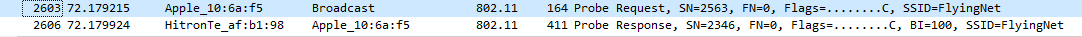
\includegraphics[width=1\textwidth]{images/cap5/probe_request_response.png}}
    \caption{Probing request e respetivo probing response}
\end{figure}


%-----------------------------------------------------------------%
\clearpage
\section{Processo de Associação}

Numa rede WiFI estruturada, um host deve associar-se a um ponto de acesso antes de enviar dados. O processo de associação nas redes IEEE 802.11 é executada enviando a trama association request do host para o AP e a trama association response enviada pelo AP para o host, em resposta ao pedido de associação recebido. Este processo é antecedido por uma fase de autenticação.

Para a sequência de tramas capturada:

\vspace{0.5cm}

\subsection{Pergunta 12}

\textbf{Identifique uma sequência de tramas que corresponda a um processo de associação completo entre a STA e o AP, incluindo a fase de autenticação.}

Nas quatro primeiras tramas, encontramos as tramas de autenticação de ambas as partes. De seguida, temos a trama de pedido de associação ao AP. Por fim, temos a trama de resposta ao pedido de associação. De notar que todas as tramas neste processo são seguidas de uma trama de Acknowledgement, que informa o último remetente que a trama foi recebida.

Na figura seguinte podemos observar um processo de associação completo entre a STA e o AP.

\begin{figure}[hbt!]
    \centering
    \frame{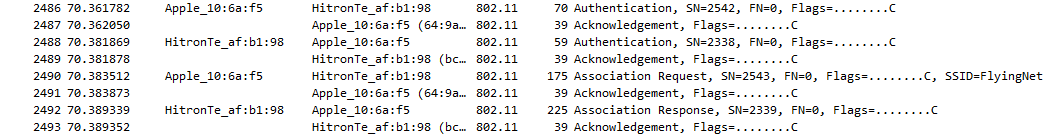
\includegraphics[width=1\textwidth]{images/cap6/processo_associacao.png}}
    \caption{Processo de associação completo}
\end{figure}

\subsection{Pergunta 13}

\textbf{Efetue um diagrama que ilustre a sequência de todas as tramas trocadas no processo.}

\begin{figure}[hbt!]
    \centering
    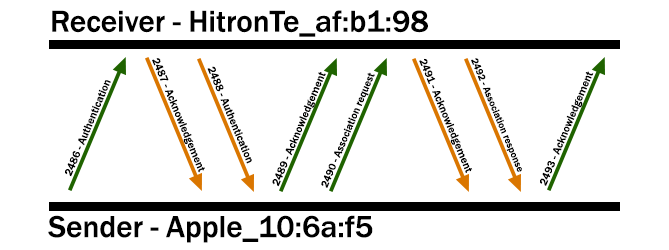
\includegraphics[width=1\textwidth]{images/cap6/diagrama_processo_associacao.png}
    \caption{Diagrama representativo do processo de associação completo}
\end{figure}


%-----------------------------------------------------------------%
\clearpage
\section{Transferência de Dados}

O trace disponibilizado, para além de tramas de gestão da ligação de dados, inclui tramas de dados e de controlo da transferência desses mesmos dados.

\vspace{0.5cm}

\subsection{Pergunta 14}

\textbf{Considere a trama de dados nº455. Sabendo que o campo Frame Control contido no cabeçalho das tramas 802.11 permite especificar a direccionalidade das tramas, o que pode concluir face à direccionalidade dessa trama, será local à WLAN?}

Como podemos ver na figura seguinte, a trama vem do Sistema de Distribuição, logo não será local à WLAN.

\begin{figure}[hbt!]
    \centering
    \frame{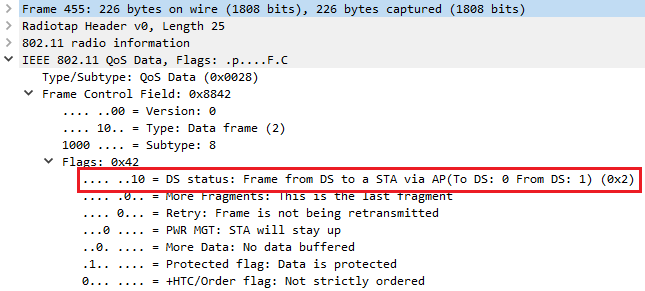
\includegraphics[width=.7\textwidth]{images/cap7/flags_DS_455.png}}
    \caption{Valor das flags DS no campo Frame Control da trama 455}
\end{figure}

\subsection{Pergunta 15}

\textbf{Para a trama de dados nº455, transcreva os endereços MAC em uso, identificando qual o endereço MAC correspondente ao host sem fios (STA), ao AP e ao router de acesso ao sistema de distribuição?}

O endereço MAC correspondente à STA é Apple\_71:41:a1, ao AP é HitronTe\_af:b1:98 e ao router de acesso ao sistema de distribuição é HitronTe\_af:b1:98.

\begin{figure}[hbt!]
    \centering
    \frame{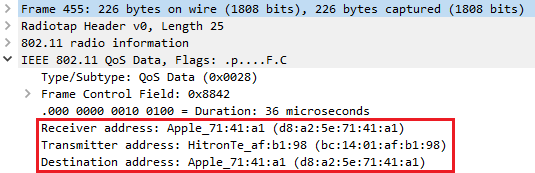
\includegraphics[width=.7\textwidth]{images/cap7/enderecos_MAC_455.png}}
    \caption{Endereços MAC da trama 455}
\end{figure}
\clearpage
\subsection{Pergunta 16}

\textbf{Como interpreta a trama nº457 face à sua direccionalidade e endereçamento MAC?}

A trama 457 tem origem na STA e vai em direção ao Sistema de Distribuição, através de um AP, ou seja, para fora da WLAN.

O endereço MAC da STA é Apple\_71:41:a1, do AP é HitronTe\_af:b1:98 e do router é HitronTe\_af:b1:98.

\begin{figure}[hbt!]
    \centering
    \frame{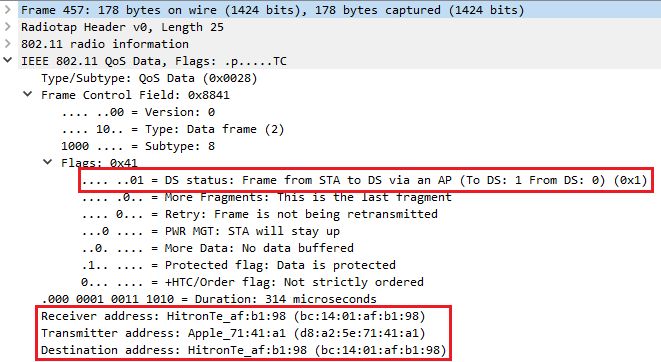
\includegraphics[width=.7\textwidth]{images/cap7/enderecos_e_ds_457.png}}
    \caption{Endereços MAC e Flags DS da trama 457}
\end{figure}

\subsection{Pergunta 17}

\textbf{Que subtipo de tramas de controlo são transmitidas ao longo da transferência de dados acima mencionada? Tente explicar porque razão têm de existir (contrariamente ao que acontece numa rede Ethernet.)}

As tramas de controlo que são transmitidas ao longo do tempo são as tramas de Acknowledgement. Estas são enviadas sempre que o recetor de uma trama de dados não detetar erros na transmissão, de forma a informar o transmissor que a trama foi enviada com sucesso. Caso o transmissor original não receba esta trama de Acknowledgement num certo intervalo de tempo, este reenvia a trama.

As tramas Acknowledgement são necessárias, pois as redes sem fios são muito mais instáveis e sujeitas a ruído do que as redes Ethernet.

\begin{figure}[hbt!]
    \centering
    \frame{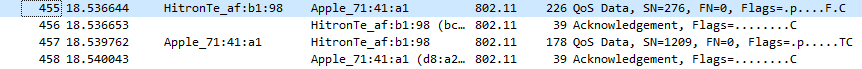
\includegraphics[width=1\textwidth]{images/cap7/tramas_controlo.png}}
    \caption{Exemplo de tramas de dados intercaladas de tramas de controlo}
\end{figure}
\clearpage
\subsection{Pergunta 18}

\textbf{O uso de tramas Request To Send e Clear To Send, apesar de opcional, é comum para efetuar "pré-reserva" do acesso ao meio quando se pretende enviar tramas de dados, com o intuito de reduzir o número de colisões resultante maioritariamente de STAs escondidas. Para o exemplo acima, verifique se está a ser usada a opção RTS/CTS na troca de dados entre a STA e o AP/Router da WLAN, identificando a direccionalidade das tramas e os sistemas envolvidos.}

Como podemos ver na figura seguinte, está a ser usada a opção RTS/CTS.

Quanto à direcionalidade das tramas, estas estão a operar localmente à WLAN, pois as flags 'To DS' e 'From DS' estão ambas a 0. Sendo assim, os sistemas envolvidos são apenas a STA (Apple\_71:41:a1) e o AP/Router (HitronTe\_af:b1:98).

\begin{figure}[hbt!]
    \centering
    \frame{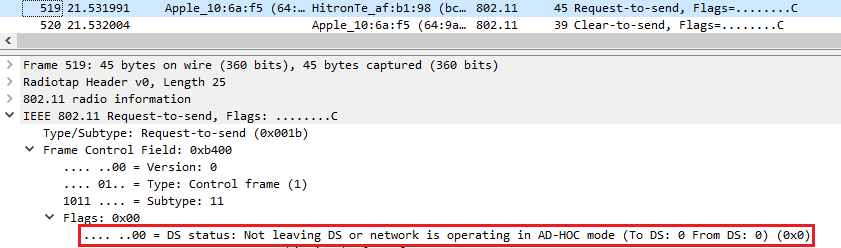
\includegraphics[width=1\textwidth]{images/cap7/rts_cts.png}}
    \caption{Exemplo de tramas 'Request To Senf' e 'Clear To Send'}
\end{figure}


%-----------------------------------------------------------------%
\clearpage
\section{Conclusão}

Neste trabalho prático, foi possível desenvolver competências acerca de redes sem fios.

Começamos por analisar as informações rádio associadas a redes sem fios.

Depois estudamos as diferenças entre Scanning Ativo e Scanning Passivo entre uma STA e um AP.

Proseguimos com o estudo do processo de associação entre um host e um AP.

Por fim, estudamos o processo de transferência de dados nestas redes sem fios.

\end{document}
